\section{Design}
\label{sec:design}
DockerGate provides a solution to auto-generate a Seccomp policy for Docker containers by performing static analysis of the executable code contained within the Docker image. The following describes its design in detail.

\subsection{Analysis Engine}

To perform static analysis, DockerGate initially requires access to the files contained within the image. To access these files it is required to instantiate the docker image to a container. We developed custom Python/Shell scripts which are  used for analysis of these files. Each script is executed in a separate container so that the results of one script do not affect the other. 

A general work flow to analyze can be described as to perform a \textbf{docker pull} on an image then execute a \textbf{docker run} on the image and execute the custom script within the new container. We collect and store the results of the scripts on the host for further analysis.We used BanyanOps~\cite{banyanops} to automate this process.

We configured the banyanops/collector framework to pull the image from Dockerhub, execute the custom scripts required to collect information on the files to be analyzed, extract the output from the docker container and save them to the host to use in the next stages of the DockerGate.

The custom scripts used to perform analysis have the following objectives:

\textit{Identify the shared libraries} : All the executables generally use library function calls of the shared libraries to interact with the system. To use any system calls, they use the wrapper functions in the form of library functions defined in the shared libraries. We developed a script to generate a list of libraries used by an executable. We use a simple approach of using “ldd” command line tool~\cite{ldd} to obtain the library dependencies of the binary files.

\textit{Identify the library function calls} : To identify the library function calls made by an executable we developed a script which uses “nm” command line tool~\cite{nm}. The nm command used with “-D” option generates a list of symbols which are not identifiable to the native execution platform.
 
The binary executable files are dynamically binded to the shared library. During execution the function calls in the binary are substituted by the corresponding native modules of execution defined in the shared library and hence in the object file they are  defined as ``Unidentified``. This makes easy to analyze the object file or binary file and use this function call for further analysis.

Mapping library functions to system calls : Libraries are defined as shared object files(.so) which contains the definition of the library functions to be loaded directly into the memory. We identified such files occurring in the container and determined the system calls for each function. We scanned all the libraries and consolidated the mapping into a single file to form a centralized database of such mapping. We used the  text section of “objdump” output~\cite{objdump} to analyze and perform the mapping of library functions and system calls. 

\subsection{Policy Generator}  

The Policy Generator is final stage in the DockerGate framework. It makes use of the output files generated by the custom scripts executed in the docker containers using Banyanops as explained in previous section.

The Policy Generator uses the files generated by the nm tool and a centralized database containing function call to system call mapping. It generates a set of system calls based on the function calls recorded by our custom scripts . This set of system calls is stored in a JSON~\cite{json} file which can further be used as a Seccomp profile.

\subsection{SYSTEM CALL DATABASE}
This is a global database generated and updated after analysis of every new shared library that is found in the docker image. The database is a JSON file which represents a list of function names format as shown in Figure \ref{fig:syscall_db}. 

\begin{figure}[t]
  \centering
  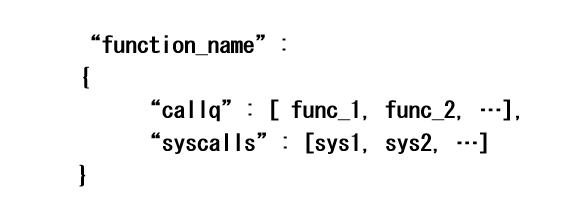
\includegraphics[width=3in]{figs/syscalldb}
  \caption{System Call Database Structure}
  \label{fig:syscall_db}
\end{figure}

The “function\_name” is the name of the library function appearing in the shared library object file. The “callq” array is a list of function calls made within the same shared object or any statically linked shared object. The “syscalls” is the list of system calls appearing in the function definition directly or indirectly. 

The system call database is generated from the analysis of the text section of the “objdump” output of the shared object file. However, the database consists of number of functions in the callq array which needs to be resolved to their respective system calls. Hence, to reduce the number of function in these callq array we resolve the functions in multiple passes by using the same database as input. Currently, we perform five passes to resolve the functions and obtain a detailed list of system calls used by the library function.

This database keeps growing with every Docker Image DockerGate analyzes. DockerGate maintains an index of all the libraries it has already analyzed. While it maintains a static database for a core set of library shared objects it analyzed in the beginning, each set of libraries a binary is linked to is added to this database. This is aimed to improve the performance of DockerGate for future runs as the mapping for a majority of shared-object libraries would already be available.

\begin{figure}[t]
  \centering
  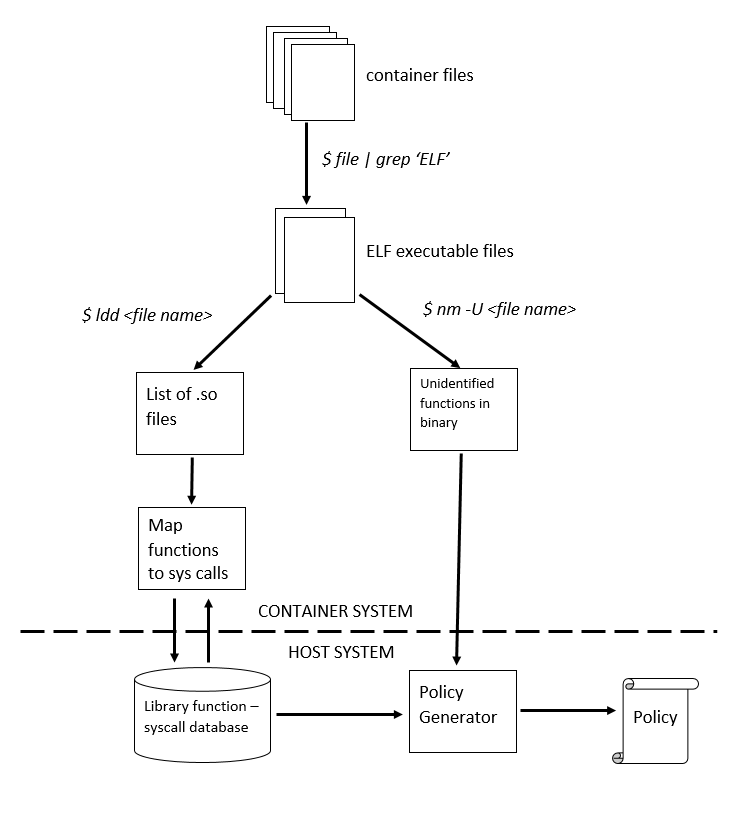
\includegraphics[width=3in]{figs/design_detail}
  \caption{A detailed design}
  \label{fig:design_detail}
\end{figure}

\subsection{WORKFLOW}

Figure \ref{fig:design_detail} shows the execution of the framework components in the container and the host system. The figure mainly covers the Analysis Engine in the DockerGate framework which performs most of its operations inside the container. 

The Analysis begins by scanning all the files inside the containers using the “file” command i.e \textbf{Stage 1}, which filters out the files identified as ELF files~\cite{elf}. ELF files are the executable binary files which contain the machine object code and references to external shared libraries used by the file.

In \textbf{Stage 2}, ELF files are processed using ldd command line tool to obtain a list of dynamically linked libraries, which are in the shared object (.so) format. These libraries are further analyzed in next stage viz Stage 3 to obtain the system calls performed in  each function call. To optimize and increase the performance of this stage, we maintain a global data set of function to system call mapping in the form of System Call Database. We also maintain a global list of library names in the `index` file which were analyzed previously for any other docker image. If any of the libraries obtained in Stage 2 exists in the `index` file, the processing for the library is skipped else the library is processed in Stage 3.

In \textbf{Stage 3}, we use the \textbf{.text} and \textbf{.plt} section of the object dump (objdump) for the shared object identified in the previous stage. The \textbf{.text} section consists of all the functions defined in that library, while the \textbf{.plt} section contains stubs of the functions that are defined in the other dynamically linked-libraries The main goal of this stage is to identify the system calls performed by each function in the library. As observed by Rauti et al~\cite{rauti2014diversification}, in Linux Architecture, a system call in the object code can be identified by a SYSCALL command. When such SYSCALL command is interpreted the system executes the system call registered in the EAX register. Linux stores numeric value of the system call in EAX. Thus, to achieve our goal, we first look for SYSCALL command in the function definition, and we backtrack the commands until we find a  `mov` command with destination register as EAX. In general we look for a instruction which satisfies the syntax “ mov 0x00,\$eax” , where 0x00 can be a numeric value or any other register. If the 0x00 is a hex equivalent of the system call number, we have identified the system call used. If the 0x00 is a register e.g. r01, r02 etc. we further backtrack the program until we find an instruction with syntax “mov 0x00, REG”, where 0x00 must be a hex value and REG is one of the register encountered as source register in the origin mov instruction with EAX. The backtracking is performed recursively in backward direction in the program until the source of the mov instruction is a hex number.

Along with the direct system calls issued by each function, it can call other functions from within the same library or any external dynamically-linked library that could in-turn eventually be required to invoke a system call. We identify these calls by the jump instructions in the programs. Some of the prominently used jump instructions are \textit{jmp, callq, jne, je} etc. When a function in the \textbf{.text} section calls a function from one of its linked libraries, it actually refers to the function stub in its \textbf{.plt} section. We leverage this fact and using basic text-processing, are able to recursively follow these function calls to the original set of system-calls, if any.

Further in Stage 3, after identifying the numeric codes of system calls, we convert them to the string equivalent or human readable format. We store this information for each function call into the System Call Database in the structure defined in Figure 2. As described previously, the System call database is refined by iterative approach to resolve the functions in the callq to be converted to system calls, thus keeping the database updated.

In \textbf{Stage 4}, we analyze the ELF files by checking which function calls are used by the particular binary files. In the object code of a binary file, the function calls to the library functions remain “unidentified”. Using the nm utility tool, with -D option, it generates a list of Unidentified symbols which are function calls to externally linked libraries. We use these functions calls and substitute them for the corresponding system calls by referring the System Call Database. This list of system calls is nothing but the system calls to be included in the seccomp policy of the docker image which are required to be allowed to execute and hence tagged under SCMP\_ACT\_ALLOW.



